% Drawing 69/06-4 -- folder 69, batch 06, archive page 103 (PDF page 104).
% Transcription: les six lettres $\bar r$, $\tilde r'$, $\bar\pi$, $\tilde r''$, $\bar r'$, $\tilde\sigma$ sur une ligne ; sous les paires, des flèches verticales vers $r$, $r'$, $r''$, $r'$, entre parenthèses, une double flèche horizontale au milieu, et deux arcs descendant vers la ligne $\pi \quad \rho \quad \sigma$
% Kind: row of six letters with arrows and arcs. Method 2 (schematic redraw from the facsimile). Status: partial.
% Notes: r-bar, r~', pi-bar, r~'', r-bar', sigma~ on a line; under the pairs, vertical arrows to (r), (r'), (r''), (r'); a double horizontal arrow in the middle; two arcs going down to the line pi rho sigma (at the bottom edge of the crop, partly cut).
% Coordinates: 1 unit = 1 mm = 1/100 of the crop width (bbox in page fractions: [0.2, 0.25, 0.65, 0.5]).
% Redrawn by Claude (claude-opus-5-5), issue #73, 2026-11-07; not checked by a human; not compiled (no TeX in the session).
% Rights: reproduces part of the work -- behind RENDER_TRANSCRIPTS, never published by itself.
\documentclass[tikz,border=3pt]{standalone}
\usepackage{amsmath,amssymb}
\usetikzlibrary{patterns,arrows.meta}
\tikzset{pencil/.style={black!45}, struck/.style={black!35}, mark/.style={circle,draw,inner sep=1.3pt}, pt/.style={circle,fill,inner sep=0.9pt}, opt/.style={circle,draw,fill=white,inner sep=1.1pt}}
\begin{document}
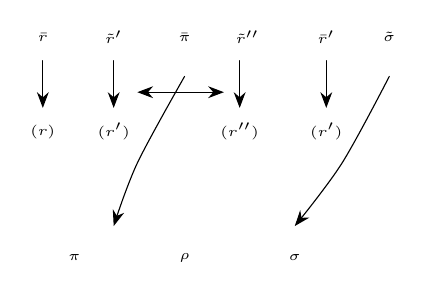
\begin{tikzpicture}[x=1mm,y=1mm,line cap=round,line join=round,font=\scriptsize]
\node[inner sep=1pt] at (28,-50) {\tiny $\bar r$};
\node[inner sep=1pt] at (37,-50) {\tiny $\tilde r'$};
\node[inner sep=1pt] at (46,-50) {\tiny $\bar\pi$};
\node[inner sep=1pt] at (54,-50) {\tiny $\tilde r''$};
\node[inner sep=1pt] at (64,-50) {\tiny $\bar r'$};
\node[inner sep=1pt] at (72,-50) {\tiny $\tilde\sigma$};
\draw[-{Stealth[length=2mm]}] (28,-53) -- (28,-59);
\draw[-{Stealth[length=2mm]}] (37,-53) -- (37,-59);
\draw[-{Stealth[length=2mm]}] (53,-53) -- (53,-59);
\draw[-{Stealth[length=2mm]}] (64,-53) -- (64,-59);
\node[inner sep=1pt] at (28,-62) {\tiny $(r)$};
\node[inner sep=1pt] at (37,-62) {\tiny $(r')$};
\node[inner sep=1pt] at (53,-62) {\tiny $(r'')$};
\node[inner sep=1pt] at (64,-62) {\tiny $(r')$};
\draw[{Stealth[length=2mm]}-{Stealth[length=2mm]}] (40,-57) -- (51,-57);
\draw[-{Stealth[length=2mm]}] plot[smooth, tension=0.55] coordinates {(46,-55) (40,-66) (37,-74)};
\draw[-{Stealth[length=2mm]}] plot[smooth, tension=0.55] coordinates {(72,-55) (66,-66) (60,-74)};
\node[inner sep=1pt] at (32,-78) {\tiny $\pi$};
\node[inner sep=1pt] at (46,-78) {\tiny $\rho$};
\node[inner sep=1pt] at (60,-78) {\tiny $\sigma$};
\end{tikzpicture}
\end{document}
